%%%%%%%%%%%%%%%%%%%%%%%%%%%%%%%%%%%%%%%%%%%%%%%%
%
% start writing
%
%%%%%%%%%%%%%%%%%%%%%%%%%%%%%%%%%%%%%%%%%%%%%%%%

\chapter{Methodology} \label{ch3_heading}

%[Introduction to contents of chapter - Data, Feature Engineering, and Modelling]
The previous chapter gave a detailed introduced money laundering, machine learning and network analytics. The chapter concluded that machine learning and network analytics could synergistically improve anti-money laundering detection processes. The methodology followed to test the project's hypothesis and answer the research question posed in chapter \ref{ch1_heading} is disclosed in the following chapter. Therefore, a detailed explanation of Figure\ref{fig:ch1_project_framework}, the high-level project overview, is provided in the chapter. The chapter is divided into three sections. The first section aims to provide all the relevant information about the data simulator (AMLSim) and how the project used it to generate the raw data for the project. The second section provides the details of the feature engineering process and its outcome - three structured data sets (network features data set, transactions feature data set, and combined features data set). The final section explains the modelling process. The section describes the models used, the pre-processing of the data, the hyper-parameter tuning process, and the model evaluation process.

\section{Data} \label{ch3_sub_heading_data}

%[What data was used? How was it obtained?]
For the projects application of network analytic's and machine learning, adequate data is needed. To obtain client transactional data from financial institutions (such as banks) is very challenging due to legal and competitive reasons \citep*{watkins2003tracking}. Therefore, obtaining actual client transactional data for research is complicated. A substitute for real-world client transactional data is synthetic data generated using a simulator. \citet*{banks1998handbook} defined simulation as being the imitation of the operations of a real-world process or system over time. Therefore, using simulation as a means to generate synthetic data that represents real-world behaviour is a sophisticated solution to obtaining the data needed for the project's purpose \citep*{lopez2016applying}. Also, simulation provides the advantages of creating different situations or scenarios, allowing the analyst to test and evaluate models under different conditions. However, the data simulator should be complex enough to mimic real-world behaviour experienced by anti-money laundering processes to conduct adequate research. For this reason, the project used a simulator developed by MIT \& IBM, called AMLSim\footnote{The GitHub page for AMLSim is found at: \url{https://github.com/IBM/AMLSim}}. AMLSim is an intricate data simulator with certain functionalities that did not apply to the project. Therefore, the project only focused on the simulator's functionalities that were useful for the project research goal. The following section explains, in detail, step one in the project's high-level overview (Figure \ref{fig:ch1_project_framework}).

%[What is AMLSim?]
AMLSim is a multi-agent simulation platform specifically created to generate synthetic data for anti-money laundering research purposes \citep*{AMLSim}. In the simulator, the agents represent bank accounts and the agent's behaviour is defined to transfer money to other agents (bank accounts). A small number of agents are tasked to participate in illegal money laundering activities. More specifically, how the ``criminal'' agents perform the money laundering is based on real-world money laundering typologies or patterns. On a high level, the functioning of the simulator is divided into two stages. The first stage generates a network of bank accounts linked by transactions. The second stage uses a secondary simulator called PaySim to produce a time series of transactions. Using Figure \ref{fig:ch3_amlsim}, these two phases of AMLSim are explained in further detail.

\begin{figure}
	\begin{center}
		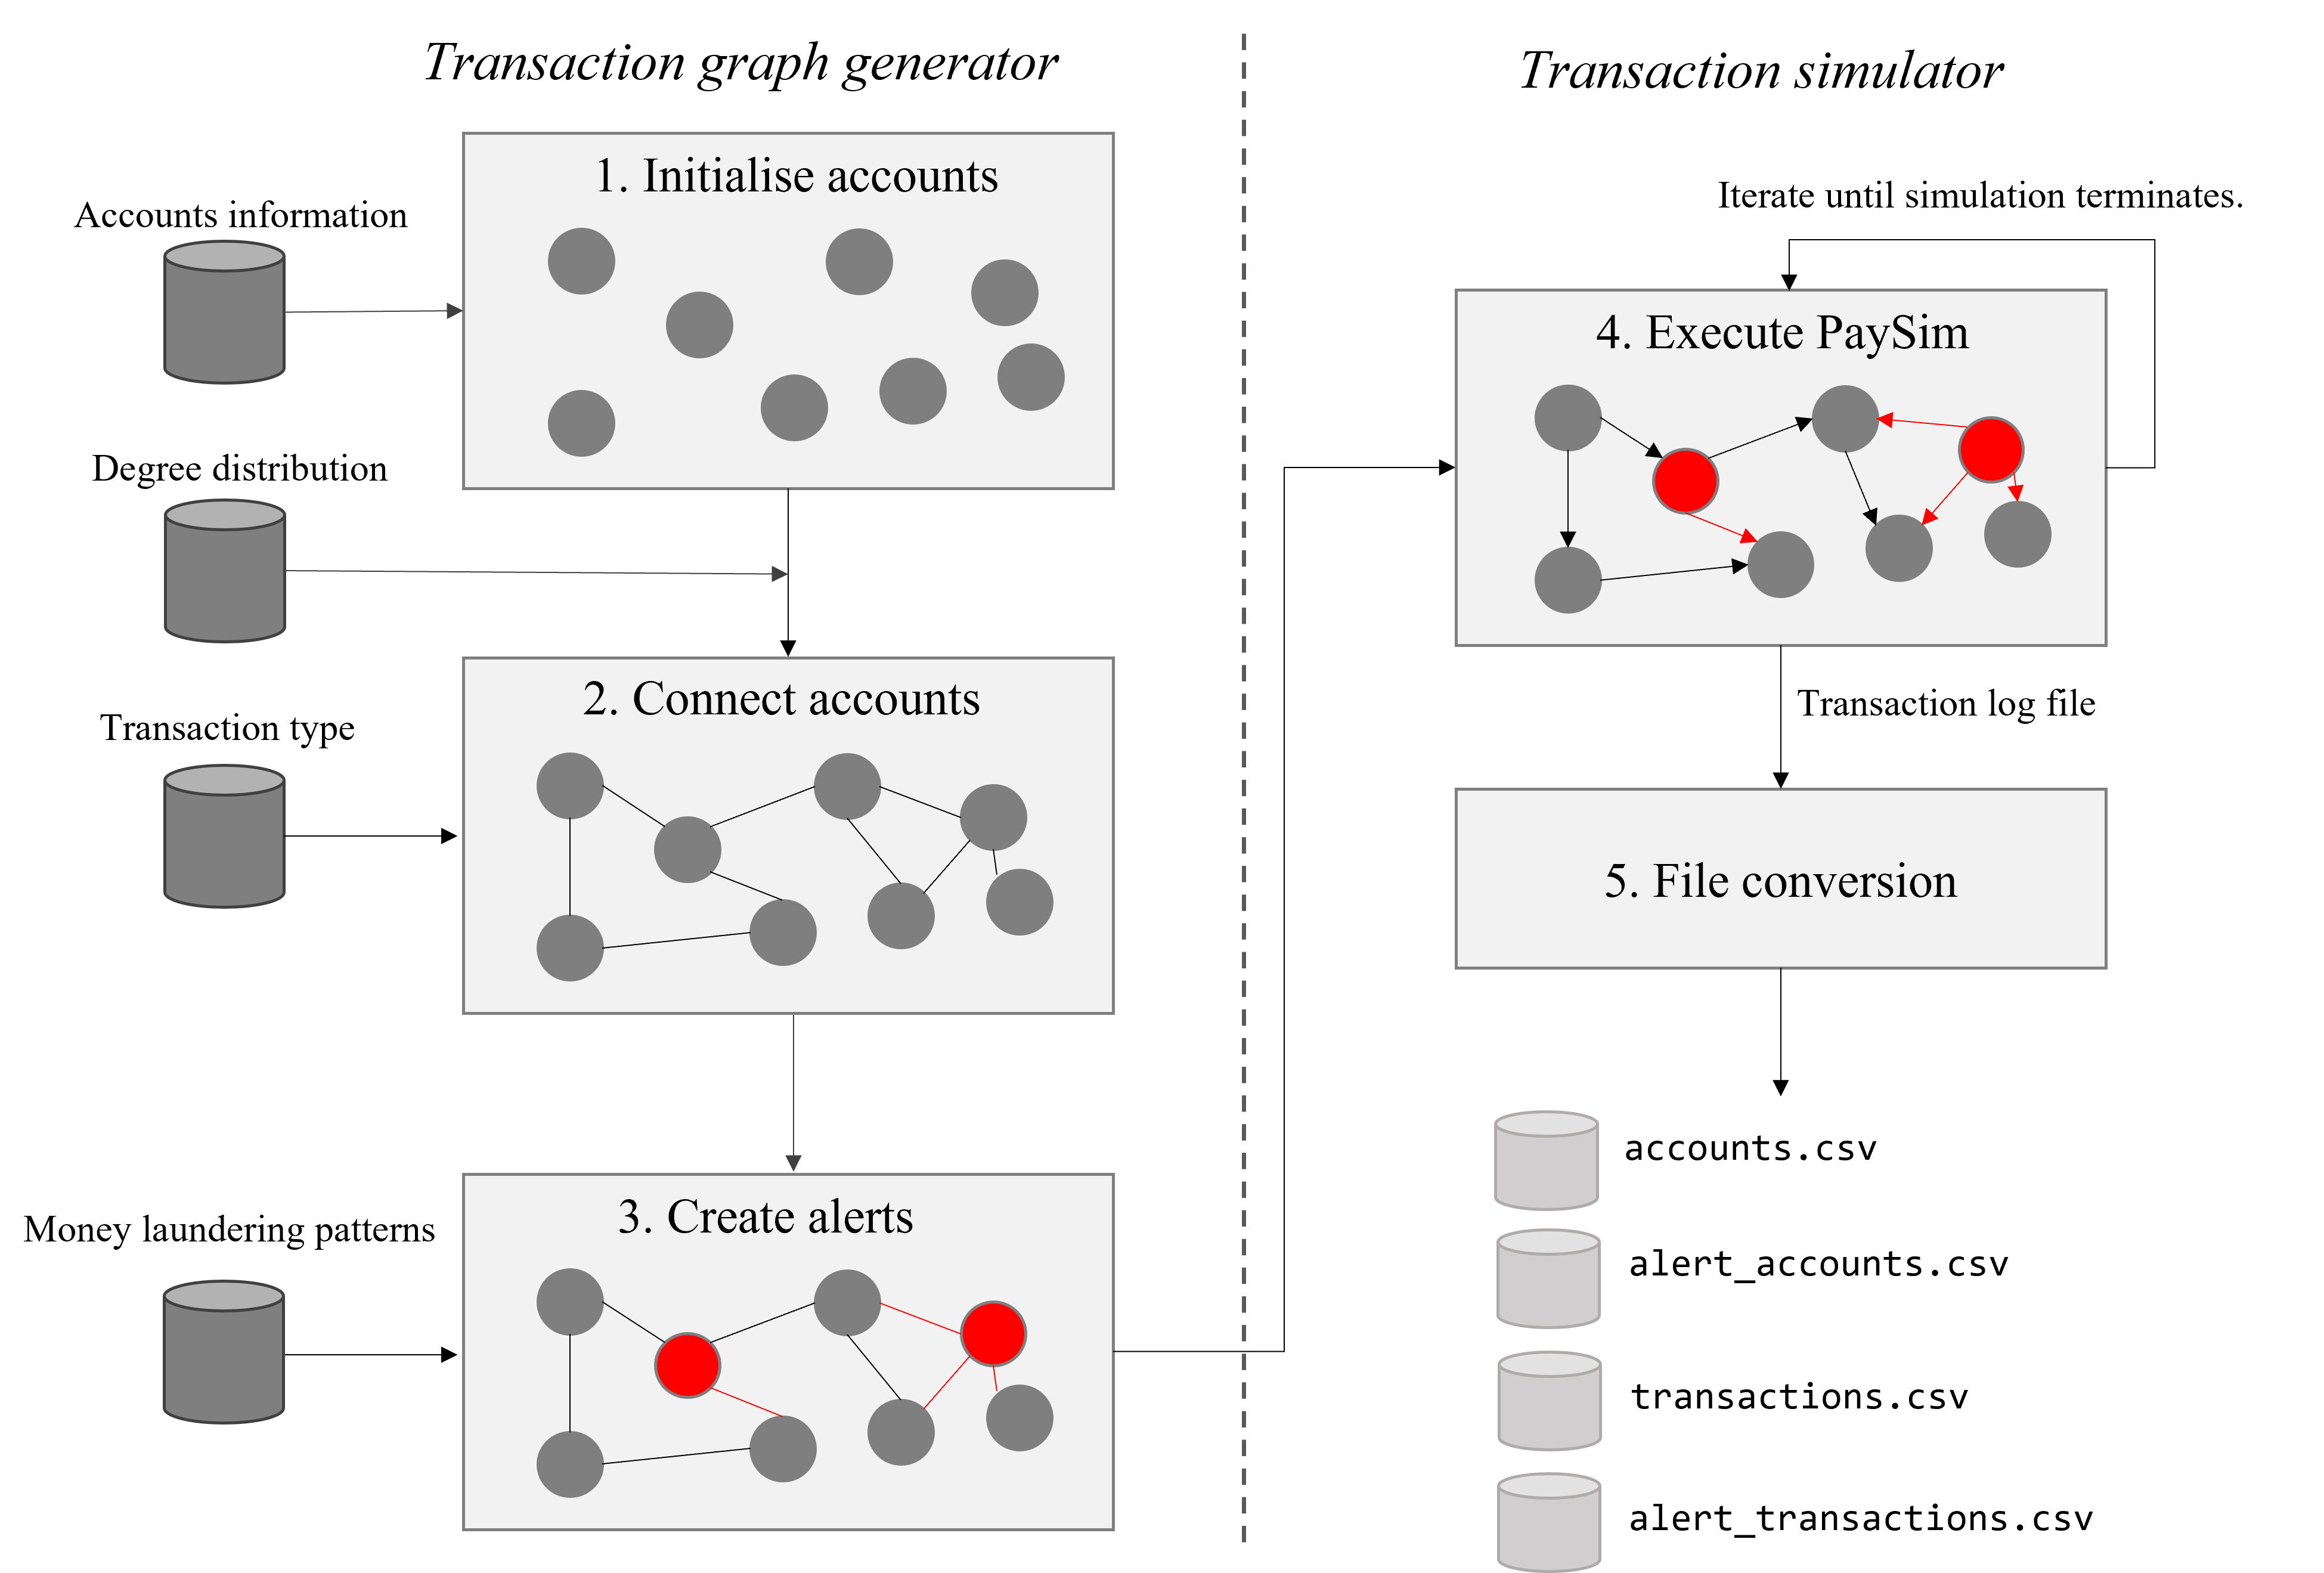
\includegraphics[scale=0.55]{fig/CH3/AML_SIm.PNG}
		\caption{A visual representation of the two stages and sub-stages in the functioning of AMLSim \citep{AMLSim, weber2018scalable, lopez2016applying}}
		\label{fig:ch3_amlsim}
	\end{center}	
\end{figure}

% [How does AMLSim work?]
% [How does AMLSim work? - inputs]
The first phase is referred to as the \textit{transaction graph generator} phase. The inputs files need to be explained before explaining this phase in more detail. The input files, along with a short description of each, are as follows:

\begin{enumerate}
    \item \textit{Transaction type}: The file specifies the type of transactions in the simulation. The types of transactions defined in the simulator are credit, deposit, wire transfer, and check. Also, the probability of each transaction type occurring is specified in the file.
    
    \item \textit{Account information}: Provides information on the bank accounts. For example, the number of accounts the simulator should generate, the initial balance for the accounts, and the behaviour the accounts should follow (discussed in further depth later on).
    
    \item \textit{Degree distribution}: Specifies the out-degree and in-degree of the bank accounts, which corresponds to the number of payments made and received by bank accounts respectfully. 
    
    \item \textit{Money laundering patterns}: The file provides the details of the money laundering activities that need to occur in the simulation. For example, the frequency of each money laundering typology (discussed in further depth later on), the time it takes to complete a money laundering activity, the money laundering amount, and the number of accounts involved in the money laundering activity.    
    
\end{enumerate}

% [How does AMLSim work? - stage 1]
The transaction graph generator consists of three sub-phases. The first sub-phase initialises a network with the properties specified in the accounts information file. In the network, the accounts are represented by vertices. After the network's vertices are generated, the second sub-phase generates the connections (edges) between the vertices according to the degree distribution and transaction type input files. The final sub-phase of the transactional graph generator is to incorporate fraudulent transactions into the network according to the metrics specified in the money laundering patterns input file. The output of the transaction graph generator is an attributed network that contains the account properties and transactional behaviour of all banking accounts (honest and money-laundering). To clarify, the transactional graph generator does not assign any values to transactions made between clients. It only specifies the characteristics or properties of the nodes (banking accounts) and edges (transactions) according to the respective input files. The values for each transaction is generated in the second phase of AMLSim - the \textit{transaction simulator}. More specifically, a time series of transactions are created using PaySim. Before discussing how the two phases merge into one another, a short introduction to PaySim is required.

% [How does AMLSim work? - stage 2 - PaySim]
PaySim is a financial simulator designed initially to simulate mobile money transactions \citep{lopez2016applying}. In short, mobile money transactions is when funds are sent or received using a mobile phone and is a type of electronic fund transfer (EFT) \citep*{money2021transfer}. The PaySim transactional simulator was built using samples of actual transactional data. As mentioned before, PaySim accomplishes the replication of real-world transactional behaviour by using agent-based simulation. An agent (represented by a bank account) is placed in an environment that requires it to make particular decisions depending on the information it receives. The agent's choice to execute a transaction is based on statistical distributions. Also, each agent has an assigned probability value, which indicates the agents' probability of performing transactions in future steps. Altogether, the \textit{input information} the agent receives, the \textit{statistical distributions} (to execute a transaction or not), and the \textit{probability value} of making future transactions were defined when PaySim was initially built. These pre-defined simulation parameters best represent the behaviour of real-world transaction transfers when presented to the agent-based modelling environment. 

% [How does AMLSim work? - stage 2 and outputs]
Now that an initial understanding of PaySim is established, the discussion can continue how it functions within AMLSim. The transaction simulator consists of three stages. These stages are essentially the stages of executing the PaySim simulator. The first stage, the \textit{initiation stage}, takes as input the attributed network, generated by the transaction graph generator, and extracts all the information required for the agent-based simulation. The second stage is the \textit{execution stage}. This stage is where the actual simulation takes place. Based on the input parameters (extracted from the attributed network), the agents will have sufficient knowledge of their role in the simulation. For example, the number of transaction's they can make in the simulation time, their initial balance, and their distributional properties (which entails the probabilities of executing a certain action). The third sub-stage is the \textit{finalisation stage}. After each agent has completed their assigned roles, the simulation is terminated, and the results are saved. Several output files are generated upon the termination of PaySim. The only output file used by AMLSim is the transaction log file. In short, the transaction log file provides a record of each transaction made and the meta-data for the transaction. Finally, the log file is converted to a more user-friendly format along with additional accounts information. The final output of the AMLSim simulation are four \texttt{csv} files: \texttt{accounts.csv}, \texttt{alert\_accounts.csv}, \texttt{transactions.csv}, and \texttt{alert\_transactions.csv}. These files would serve as the raw data for the project. The exploratory data analysis (EDA) provides a more detailed explanation of these raw data files, discussed later in the section. 

%[What input parameters were used, in AMLSim, to generate the data for the project?]
Since an understanding of AMLSim is established, more focus can be placed on the contents of the input files (transaction type, account information, degree distribution, and money laundering patterns) specified for the project's purposes. Establishing which input parameters to use for the project research question was a significant challenge due to the infinite possible combinations of input parameters. There is also no clear consensus found in literature on what input parameters should be used to generate baseline anti-money laundering data \citep{pareja2020evolvegcn, AMLSim, weber2018scalable}. Luckily, \citet{AMLSim} defined several fixed input parameter folders that generate anti-money laundering data specifically compiled for testing machine learning models. Within the fixed input parameter folders are the respective simulator input files. The fixed input folders used for the training data set and the testing data set was the ``\texttt{10K}'' and ``\texttt{1K}'' folders, respectively. The only difference between the two input folders is the number of accounts used in the simulation. The ``\texttt{10K}'' folders generates approximately 10 000 accounts and the ``\texttt{1K}'' folder generates approximately 1000 accounts. The project will provide more details on the training and testing data set in section \ref{ch3_sub_heading_modelling}. Furthermore, except for the money laundering patterns input file, all the default settings for each input file were used. To understand the alteration made to this input file, an explanation of the normal and money laundering typologies defined within AMLSim needs to be established first.
% [money laundering and normal typology's - inputs to the project]

AMLSim has various normal and money laundering typologies defined. The normal typologies are \textit{periodical}, \textit{forward}, \textit{single}, \textit{fan-in}, \textit{fan-out}, and \textit{mutual}. Firstly, the \textit{periodical} typology is when account X sends funds to account Y on some periodical basis (weekly, monthly, etc.). The \textit{forward} typology is when account X transfers funds to account Y, and then account Y forwards the funds to account Z. A \textit{single} typology is when account X makes a transfer to account Y. The \textit{fan-in} and \textit{fan-out} typologies refer to when an account receives funds from multiple other accounts or when an account makes transfers to multiple other accounts, respectively. The final normal typology, \textit{mutual}, refers to when account X makes a transfer to account Y and then, shortly after some time, receives the funds back from account Y. The money laundering typologies incorporated in AMLSim are more complicated than the normal typologies. The money laundering typologies are \textit{cycle}, \textit{fan-in}, \textit{fan-out}, \textit{gather-scatter}, \textit{scatter-gather}. The \textit{cycle} typology occurs when an account transfers funds to another account, and after several other transfers involving other accounts, the funds return to the origin account. For example, account X transfers funds to account Y, and account Y transfers the funds to account Z and account Z transfers the funds back to account X (completing the ``cycle''). The \textit{fan-out} and \textit{fan-in} money laundering typologies are equivalent to that explained in the normal typologies; however, the \textit{gather-scatter} typology combines the fan-in and fan-out typologies after each other (vice versa for the \textit{scatter-gather} typology).      

% [changed values to money laundering patterns file - inputs to the project]
Now that an understanding of the normal and money laundering typologies has been established, the alteration of the default values of the money laundering patterns input file can be explained. Initially, the input file only had three money laundering typologies specified (fan-in, fan-out, and cycle). It was decided to include \textit{all} other money laundering typologies since the project research goal was to investigate how network or graph derived features impacts a classifier's performance in detecting money laundering activity among banking accounts, in \textit{general}, and not focusing on a specific set of money laundering typologies. Therefore, the added money laundering typologies were: gather-scatter and scatter-gather.

% [How did the raw data look? - EDA raw data]
After correctly configuring all input files, the AMLSim simulator was executed \textit{twice}. Firstly, to generate the training raw data (using the ``\texttt{10K}'' input folder) and a secondly to generate the testing data (using the ``\texttt{1K}'' input folder). The only difference between the two input folders is the number of accounts initialised in the simulation. Furthermore, the features generated in the output files are identical. As mentioned before, AMLSim produces the following \texttt{csv} files: \texttt{accounts.csv}, \texttt{alert\_accounts.csv}, \texttt{transactions.csv}, and \texttt{alert\_transactions.csv}. The  project did not directly use the \texttt{alert\_accounts.csv} and \texttt{alert\_transactions.csv} files in the feature engineering phase (discussed in section \ref{ch3_sub_heading_feature_engineering} ); however, they were included in the EDA conducted of the outputted raw data files. An exploratory data analysis is an essential part of any data analysis \citep*{wickham2016r}. There is no formal process or strict rules when conducting exploratory analysis. In short, the goal of an EDA is to develop an understanding of the data \citep{wickham2016r}. A high-level explanation of the process of the EDA conducted of the raw data files was: i) examining the quality of the data generated by the simulator, ii) to observe if the input parameters specified was reflected in the data, and iii) to generate questions about the data that could produce helpful insights. At first glance, there were multiple features in each raw data table that contained only singular values (repetitions of the same values). These features were removed since they would not be beneficial to analysis. There were also other reasons why some variables were excluded from the analysis. Table \ref{tab:ch3_raw_features_removed} in appendix \ref{app_1} summarises all the raw data features excluded from the analysis and why. After the data cleaning exercise, the investigation of the data continued. For each raw data table (training data set and testing data set), the project investigated the following: i) basic table characteristics (for example, the number of rows/columns, data type of each variable, etc.), ii) missing data profile (how many instances of each feature was missing), iii) Uni-variate statistics (histograms - continuous variables, frequency bar charts - discrete variables ), and iv) Bi-variate distributions (box and whisker diagrams). All statistics and visualisations generated for the EDA were done for the generated training and testing raw data files. 

% [Training set - EDA raw data]
 There were 12 043 accounts and 655 433 transactions from the raw training data set. From these accounts, 782 participated in money laundering activity ($\approx 6.5\%$ of all accounts), and 626 transactions were classified as fraudulent ($\approx 1\%$ of all transactions). Figure \ref{fig:ch3_raw_eda_train_alrt_trans_sum} shows four plots generated from the \texttt{alert\_transactions.csv} file. The bottom-left plot shows that the cycle money laundering typology is the most frequent among illicit transactions, and the gather-scatter is the least. Figure \ref{fig:ch3_raw_eda_train_alrt_trans_tx_distr} shows the distributional properties of the transaction amount (\texttt{base\_amt}) for each money laundering typology. Generally, the transactions are widely distributed among all money laundering typologies, except for the scatter-gather typology, which has much more concentrated amounts between approximately \$170 and \$190. The bottom-left plot in Figure  \ref{fig:ch3_raw_eda_train_acct_sum} shows a box and whiskers plot of the opening account balance (\texttt{initial\_deposit}) for fraudulent and non-fraudulent accounts. The two distributions seem identical for both fraud and non-fraud clients.
 
% [Testing set - EDA raw data]
There were 1446 accounts and 108 684 transactions in the raw testing data set. From these accounts, 72 participated in money laundering activity  ($\approx 5\%$ of all accounts), and 52 transactions were classified as fraudulent ($\approx 0.5\%$ of all transactions). The EDA also generated the same type of figures displayed for the training data (Figures \ref{fig:ch3_raw_eda_test_alrt_trans_sum}, \ref{fig:ch3_raw_eda_test_alrt_trans_tx_distr}, and \ref{fig:ch3_raw_eda_test_acct_sum}) for the test data. These figures are displayed in appendix \ref{app_2}. Overall, very similar characteristics are observed in the raw test data set. For example, the money laundering typology least frequent among illicit transactions is the gather-scatter typology (Figure \ref{fig:ch3_raw_eda_test_alrt_trans_sum}). Also, the transaction amount distributions for the money laundering typologies are widely spread, except for the scatter-gather typology (Figure \ref{fig:ch3_raw_eda_test_alrt_trans_tx_distr}). Finally, a slight difference between the initial balance means of fraudulent accounts and non-fraudulent accounts is observed (Figure \ref{fig:ch3_raw_eda_test_acct_sum}).


\begin{figure}
	\begin{center}
		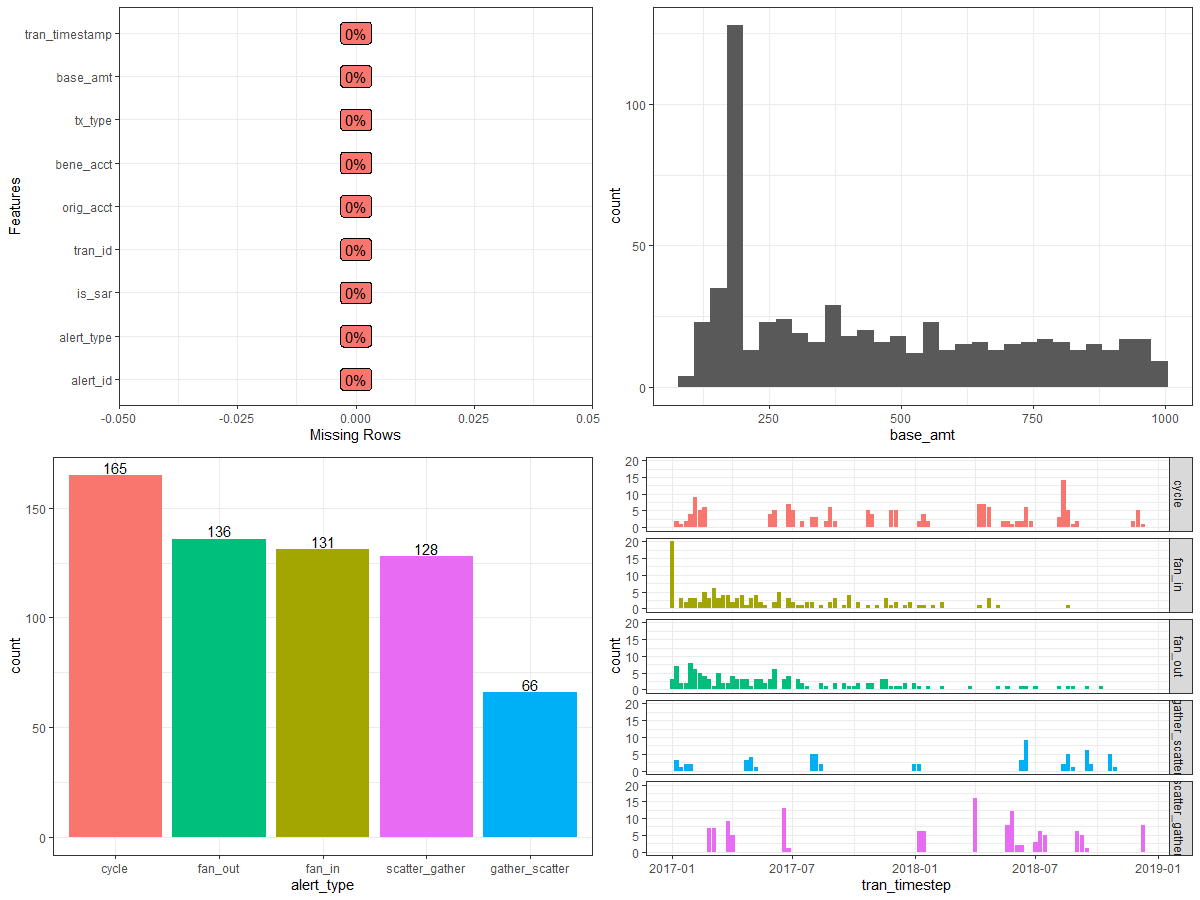
\includegraphics[scale=0.5]{fig/CH3/train_alrt_trans_summary.png}
		\caption{Example of the visualisations generated during the EDA of the training \texttt{alert\_transactions.csv} file. (top-left) The missing values profile. (top-right) Histogram of the transaction amount (\texttt{base\_amount}). (bottom-left) Frequency bar chart of the occurrences of different money laundering typologies (\texttt{alert\_type}) among the account transactions. (bottom-right) A timeline plot of when the different money laundering typologies occurred.}
		\label{fig:ch3_raw_eda_train_alrt_trans_sum}
	\end{center}	
\end{figure}

\begin{figure}
	\begin{center}
		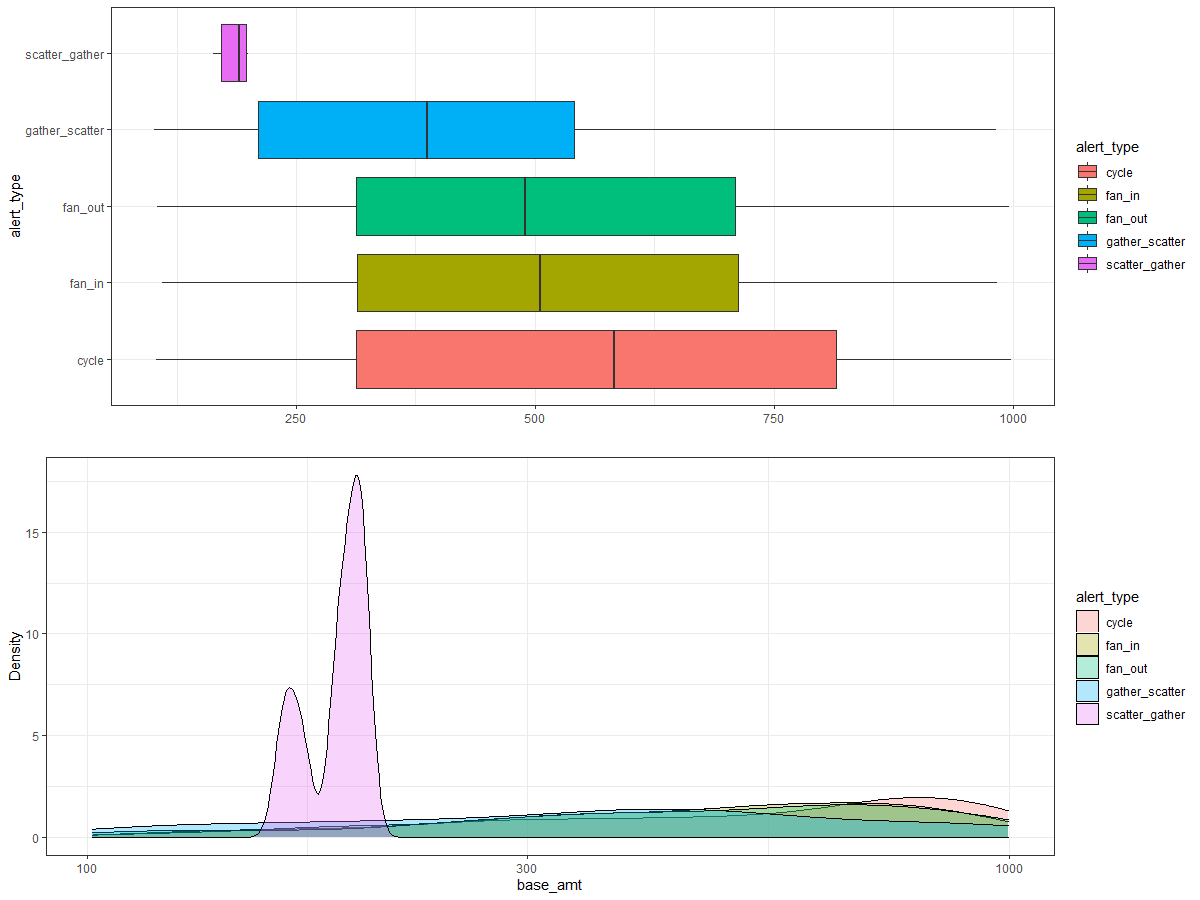
\includegraphics[scale=0.5]{fig/CH3/train_alrt_trans_tx_amount_alert_type_distribution.png}
		\caption{Both plots show the transaction amount distribution (top - box and whiskers and bottom - density plot) of transactions that were classified as being money laundering transactions for the training \texttt{alert\_transactions.csv} file.}
		\label{fig:ch3_raw_eda_train_alrt_trans_tx_distr}
	\end{center}	
\end{figure}

\begin{figure}
	\begin{center}
		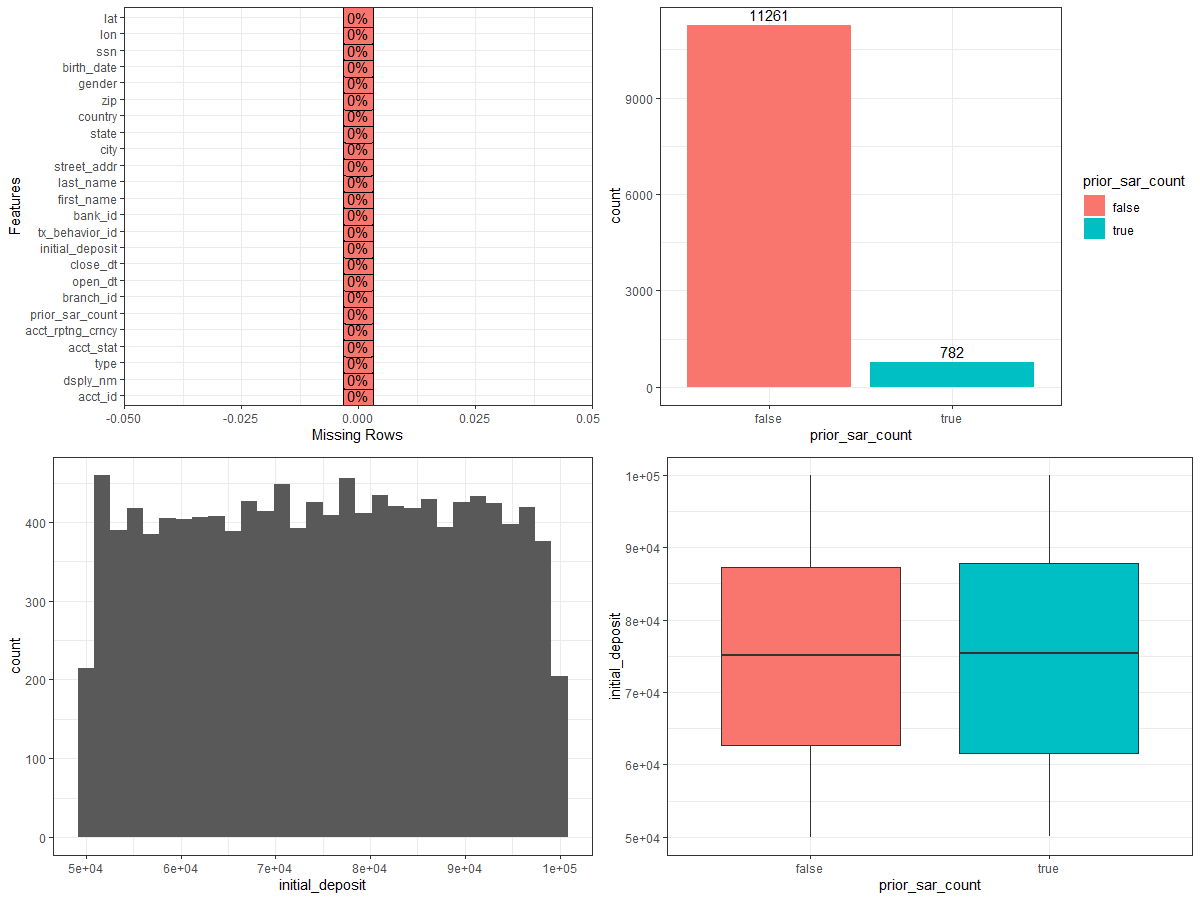
\includegraphics[scale=0.5]{fig/CH3/train_acc_summary.png}
		\caption{Example of the visualisations generated during the EDA of the training \texttt{accounts.csv} file. (top-left) The missing values profile. (top-right) Frequency bar chart of accounts that did and did not participate in money laundering activity. (bottom-left) Histogram of the accounts initial balances (\texttt{initial\_deposit}.  (bottom-right) A box and whiskers plot showing money laundering and honest accounts' initial deposits.}
		\label{fig:ch3_raw_eda_train_acct_sum}
	\end{center}	
\end{figure}

\section{Feature engineering} \label{ch3_sub_heading_feature_engineering}

%[Introduction to feature engineering section]
The previous section explained the raw data generation process (step one in Figure\ref{fig:ch1_project_framework}). This section  provides the details of the feature engineering process - how the raw data was used to create new features. The section will explain how each of the three structure data sets was constructed: \textit{network feature} data set, \textit{transactional feature} data set, and \textit{combined feature} data set. The previous section  mentioned that AMLSim was used to generate two raw data sets, a training data set and a testing data set. The feature engineering process for both data sets was identical. Therefore, both raw data sets will be referred to as the ``raw data set'' for this section.  
As mentioned in the previous section, the output of AMLSim is four raw data files. However, the project used only two of the files (\texttt{transactions.csv} and \texttt{accounts.csv}) for the feature engineering process. The finalised raw data, used as input for the feature engineering process, is displayed in Table\ref{tab:ch3_raw_data_final}. 

\begin{table}
\begin{tabular}{cll}
\hline
\multicolumn{1}{l}{\textbf{Raw data table}} & \textbf{Feature name} & \textbf{Description}                                                                                          \\ \hline
\multirow{3}{*}{\texttt{accounts.csv}}               & \texttt{acct\_id}              & ID number of client account.                                                                                  \\
                                            & \texttt{prior\_sar\_count}    & \begin{tabular}[c]{@{}l@{}}If the account has been involved in any money \\ laundering activity.\end{tabular} \\
                                            & \texttt{initial\_deposit}     & \begin{tabular}[c]{@{}l@{}}The initial balance when the client created \\ the account.\end{tabular}           \\ \hline
\multirow{7}{*}{\texttt{transactions.csv}}           & \texttt{tran\_id}              & ID number for transaction.                                                                                    \\
                                            & \texttt{origin\_acct}          & The account ID that makes the funds transfer.                                                                 \\
                                            & \texttt{bene\_acct}           & The account ID that receives the funds transfer.                                                              \\
                                            & \texttt{base\_amt}             & The transaction amount transferred.                                                                           \\
                                            & \texttt{tran\_timestamp}       & The date and time the transaction occured.                                                                    \\
                                            & \texttt{is\_sar}              & \begin{tabular}[c]{@{}l@{}}If the transaction is a money laundering \\ transaction.\end{tabular}              \\
                                            & \texttt{alert\_id}             & \begin{tabular}[c]{@{}l@{}}The ID indicating the type of money laundering \\ typology occurred.\end{tabular}  \\ \hline
\end{tabular}
\caption{The Table provides the finalised raw data tables used in the project (for both the testing and the training set). In addition, the table details the raw data table name, the features of the raw data table and a short description of each.}
\label{tab:ch3_raw_data_final}
\end{table}

%[Generation of Network feature data set - undirected weighted graph]
The network metrics chosen for the \textit{network feature data set} was the most popular network metrics applied for some anti-money laundering application found in literature \citep{boccaletti2006complex, zanin2016combining, colladon2017using, drezewski2015application, van2017gotcha}. \citet{baesens2015fraud} was specifically helpful in defining the network metrics. Also, they provided toy examples that the project used to validate and verify the output of the network extraction functions used to generate the network feature data set. The network feature data set was the first structured data set generated using the raw data. Firstly an undirected network was constructed using the raw data files. The vertices in the networks would represent the accounts, and the edges would represent the transactions made between accounts. Since an account can make (receive) multiple transactions to (from) another account, multiple edges exist in the network. Therefore, the network is a multigraph. Also, the network constructed did not contain any loops (accounts transferring money to themselves). Then the undirected network, containing multiple edges, was simplified to an \textit{undirected weighted network} by aggregating the transactions amounts between two vertices and collapsing the multiple edges between two nodes into a single edge. For example, $w_{AB}$ is calculated by:

$$\sum_{i = 1}^{k}TX(l_{AB})_i + \sum_{j=1}^{d}TX(l_{BA})$$

where $TX()$ is a function that extracts the transaction value of the $i^{th}$ or $j^{th}$ edge $l_{AB}$ or edge $l_{BA}$, respectively. Here, the values $k$ and $d$ represent the number of edges from node $A$ to $B$ and $B$ to $A$, respectively. Therefore, the weights between adjacent nodes represent  the total transactional amount exchanged between the nodes. Recall that a weight should be defined such that it serves as an indication of the strength of the relationship between neighbouring nodes. Therefore, the project assumed that nodes (accounts) with a high total transaction exchange amount exhibit a strong relationship. After the undirected weighted network was defined, it was divided into its graph components. It was decided to only consider graph components of size $N > 2$, due to graph components with size $N=1$ or $N=2$ producing \texttt{NA} and \texttt{Inf} values for multiple of the chosen network metrics (for example, transitivity, triangles, closeness centrality, etc.). Also, graph components of size $N<3$ seem to be either a client account recently opened (which made one or two transactions) or accounts that exhibit minimal financial activity (possibly a client that has other bank accounts). After extracting the graph components, the extraction of the network metrics could commence. Features 1-22 in Table \ref{tab:ch3_network_features} in appendix \ref{app_1} provides the list of all the network-related features extracted from each undirected weighted graph component and a short description of each. 

%[Generation of Network feature data set - directed graph]
After the network metric extraction from the undirected weighted graph components was complete, a \textit{directed network} was constructed using the raw data files. A directed network was constructed to extract useful network information concerning the \textit{direction} of transactions (which was not captured in the undirected weighted network). The process of extracting the network metrics from the directed graph was similar to the undirected weighted graph. After constructing the directed graph, the graph was divided into components of size $N>2$ (for the same reasons as mentioned before). Then for each graph component, its network metrics were extracted. Features 23-28 in Table \ref{tab:ch3_network_features} in appendix \ref{app_1} provides the list of all the network-related features extracted from each directed graph component and a short description of each. Finally, the network feature data set was constructed by joining the features extracted from the undirected weighted network and the directed network using the \texttt{acct\_id} as the primary joining key. Table \ref{tab:ch3_network_features} provides the finalised features for the network feature data set. 

%[Generation of transaction data set]
The generation of the \textit{transactional feature data set} was much more straightforward. The goal was to construct as many useful features from the raw data sets, that could provide a machine learning model with the right inputs to identify hidden patterns within the data. Therefore, the project applied no network analytic's to construct the transactional feature data set. \citet{visserdetection} also used the AMLSim simulator to generate data for anti-money laundering research purposes. However, their approach focused on using transactional-based features to predict illicit activity. Therefore, most  transactional features were derived from their work. Table \ref{tab:ch3_trans_features} in appendix \ref{app_1} provides the list and a description of all the transactional features generated for the transactional feature data set.      

%[Generation of combined data set and conclusion of section]
The final structured data set is the combined feature data set. This data set contains all the features generated during the feature engineering process. Therefore, the combined data set contains network features and transactional features. The combined feature data set can be visualised when the features from Tables \ref{tab:ch3_network_features} and \ref{tab:ch3_trans_features} are joined by using the \texttt{acct\_id} as the primary joining key.  

\section{Modelling} \label{ch3_sub_heading_modelling}

The previous section explained how all three structured data sets were constructed using the raw data (generated using AMLSim). To clarify, the project applied the feature engineering process for both the training and testing raw data sets. Therefore, there is a training and testing set for each data set (network feature data set, transactional feature data set, and combined feature data set). This section tests the project research hypothesis by using these structured data sets as input to two different classifiers. The first classification model will be a \textit{logistic regression} model, and the second classifier will be a \textit{neural network} model. The classification task is to predict, based on the given input features (network, transactional, or combined), if an account is participating in money laundering activity or not (the \texttt{is\_fraud} feature). A brief introduction to each classification model, the data pre-processing, hyper-parameter tuning and training, and evaluation of model performance are detailed in the section.               

% [Introduction - logistic regression]
Linear regression is a well established technique and has been studied for an extended period. While linear regression might seem like a monotonous method, compared to some modern-day statistical learning approaches, it remains an effective and extensively used statistical learning method \citep{james2013introduction}. For example, it can be argued that in the case where unknown target function $f$, is highly complex, a simple hypothesis set, $\mathcal{H}_{simple}$ would provide a better approximation $\hat{f}$, as to try to match the complexity of $f$, with a more complex hypothesis set $\mathcal{H}_{complex}$ \citep{abu2012learning}. Linear regression is a useful tool for predicting a quantitative response; however, the model can be easily extended to predict a qualitative response. This class of model is the \textit{logistic regression model}. The logistic regression model is more concerned with modelling the \textit{probability} that $y_i$ belongs to a certain class \citep{james2013introduction}. A short introduction to the logistic regression model follows. Suppose we have a binary classification problem with response:


$$y_i = \left \{\begin{array}{ll} 
 1 & \pi_i \geq \theta  \\ 
 0 & \pi_i < \theta  
\end{array} \right.
$$

where $\pi,\theta \in [0,1]$ and the threshold is assumed to be $\theta = 0.5$. If we would like to model the relationship between $\pi_i = Pr(y_i = True|\boldsymbol{x}_i)$ and $\boldsymbol{x}_i$ using the logistic regression model we need to start with the linear equation (as  \citet*{et2020analytics} explains):

$$\eta_i = \boldsymbol{x}_i^T\boldsymbol{w}$$

The idea is to define a ``link'' function, $h$, that maps $\eta \in \mathcal{R}$ to $[0,1]$. There are various choices for the function $h$. It can be the ``Logit'' function, ``Probit'' function, or complimentary log-log function. Suppose we use the ``Logit'' function as our ``link'' function, then the relationship between the linear component $\boldsymbol{x}_i^T\boldsymbol{w}$  and $\pi_i$ is expressed as:

$$\pi_i =  \frac{e^{\boldsymbol{x}_i^T\boldsymbol{w}}}{1 + e^{\boldsymbol{x}_i^T\boldsymbol{w}}}$$

Therefore, given the parameter vector $\boldsymbol{w}$ values, we may ``predict'' a probable result for a given set of features $\boldsymbol{x}_i$. To obtain suitable values for $\boldsymbol{w}$ we use the \textit{maximum likelihood} method. More specifically, we maximise the log-likelihood function:

\begin{equation}
    l(\boldsymbol{w}) = \sum_{i=1}^{n}(y_ilog(h^{-1}(\boldsymbol{x}_i^T\boldsymbol{w})) + (1-y_i)log(h^{-1}(\boldsymbol{x}_i^T\boldsymbol{w}))
\label{ch3_log_lik_eq}
\end{equation} 
 
After an suitable numerical optimisation routine is defined and a estimation of the weight parameter $\boldsymbol{\hat{w}}$ is defined, then the probability predictions are $\hat{\pi} = h(\boldsymbol{x}^T\hat{\boldsymbol{w}})$.

% [ Model definition - logistic regression]
Logistic regression models are capable of dealing with categorical predictors. Luckily, all three structured data sets had numerical predictors. Therefore, before any logistic regression models were implemented, the data pre-processing was to \textit{standardise} the data. Al three structured data sets were standardised since some of the features were not of the same unit of measure. Standardisation is recommended as an effective tool to solve this problem \citep{james2013introduction}. Furthermore, all logistic regression models were defined using the ``Logit'' function as the chosen ``link'' function. The optimisation routine or learning algorithm used to approximate a maximum for the log-likelihood function (Equation \ref{ch3_log_lik_eq}) was the Iterative Weighted Least Squares method (IWLS). This logistic regression model was applied to each structured training data set along with an L1 regularisation penalty. 

% [Regularisation - logistic regression]
Regularisation is a valuable technique for controlling a model's flexibility/complexity \citep{et2020analytics}. Managing the complexity of a model, using some regularisation mechanism, can also improve the models' ability to \textit{generalise} out of sample. Therefore, the model achieves a low in-sample error $E_{in}$ (typically the training error), but also a low out-of-sample error $E{_{out}}$ (typically the validation error). The only challenge in introducing some regularisation mechanism is the additional hyper-parameter(s) that must be ``tuned''. In applying \textit{L1 regularisation}, the only hyper-parameter that needs to be specified is the \textit{regularisation factor}, $\lambda$. In approximating the best $\lambda$ for each data set, the project used the process of \textit{K-fold-cross-validation}. Using $K = 10$ is an appropriate choice for the number of folds since it represents a suitable balance between unbiased estimation (leave-one-out cross-validation) with large variation and biased estimation with low variation but at the risk of overestimating the out-of-sample performance since a large portion of
the data is used to fit the model \citep{et2020analytics, friedman2001elements}. Figure \ref{fig:ch3_lr_lambda_cv_network} illustrates the ten-fold cross-validation applied to the logistic regression models with the L1 penalty for the network feature data set. The identical plots for the transactional feature data set and combined feature data set are illustrated in Appendix \ref{app_1} Figure \ref{fig:ch3_lr_lambda_cv_trans} and Figure \ref{fig:ch3_lr_lambda_cv_all}, respectively. Also, there are two vertical dashed lines in the plots mentioned above. The first line (from the left) indicates $\lambda_{min}$. At this $\lambda$ value, the MSE is at its minimum. The second line indicates $\lambda_{1 SE}$ which is the biggest $\lambda$ value that is one standard error from the $\lambda_{min}$. The $\lambda_{1 SE}$ was the chosen regularisation factor value for all logistic regression models, which had L1 regularisation applied. This decision was made because the regularised model with the higher regularisation factor ($\lambda_{1 SE}$) is, the more ``penalised'' model and, therefore, less complex. The simplest model that delivers similar performance to the best model is often the better choice \citep{friedman2001elements}.      

% [Threshold selection - logistic regression]
The \textit{threshold value} ($\theta$) was briefly mentioned in the introduction of the logistic regression model. The value of the threshold parameter determines the mapping from the predicted probability value, $\hat{\pi_i}$ to the respective class. For most classification problems, the default value for the threshold is 0.5. However, if the classification problem has \textit{high class imbalances}, such as in the project, then the default threshold can produce poor classification performance \citep*{jason2016brownlee}. Therefore the project used two methods in determining the threshold value for each logistic regression model defined. The first method was finding the optimal threshold according to the \textit{Receiver Operating Characteristic} curve (ROC). In short, the ROC curve plots a models performance for a range of threshold values where the false-positive rate ($FPR$) is shown on the x-axis and the true-positive rate ($TPR$) is shown on the y-axis. The optimal threshold value, according to the ROC curve, is the threshold value that produces the maximum \textit{Geometric Mean} ($G_{mean}$). The G-mean is calculated by: $G_{mean} = \sqrt{TPR\times(1-FPR)}$. This point on the ROC curve is usually found in the upper left side of the curve. The second method was finding the optimal threshold value according to the \textit{precision-recall curve}. In short, \textit{precision} ($p_r$) is the ratio of the number of true positives divided by the sum of the true positives, and false positives and \textit{recall} ($r_c$) is the ratio of the number of true positives divided by the sum of the true positives and the false negatives. Similarly to the ROC curve, the precision-recall curve plots a models performance for a range of threshold values where the recall is shown on the x-axis and the precision is shown on the y-axis. The optimal threshold value, according to the precision-recall curve, is found at the threshold value where the \textit{F-measure} or \textit{F1-score} ($F_1$) is at its maximum. Equation \ref{ch3_f1_eq} shows how the F1-score is calculated. Figure \ref{fig:ch3_lr_thresh_roc_lasso_network} and Figure \ref{fig:ch3_lr_thresh_pr_lasso_network}illustrate the optimal threshold value chosen according to the ROC curve and precision-recall curves for the logistic regression model with an L1 penalty applied to the network training data.  

  % 10-Fold cross-validation (lambda - network data)
\begin{figure}
	\begin{center}
		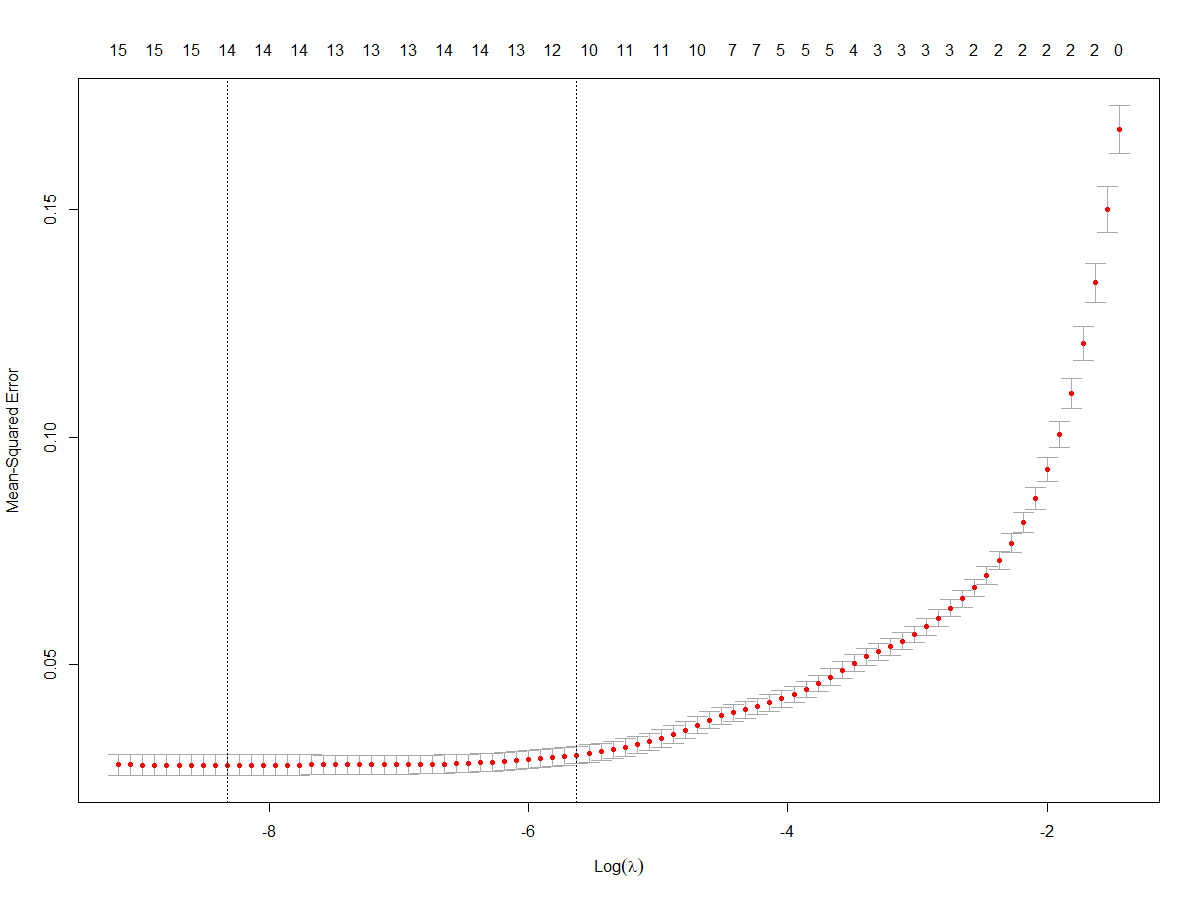
\includegraphics[scale=0.45]{fig/CH3/cv_lambda_network.png}
		\caption{Ten-fold cross-validation mean square error (MSE) for the L1 regularised logistic regression model applied to the network feature data set. The vertical dashed line on the left is the $log(\lambda)$ value of where the MSE is at its minimum and the vertical on the right is the largest $log(\lambda)$ value such that the MSE is within one standard error of the minimum MSE. Also, the plot illustrates at the top, the number of positive weights $\boldsymbol{w} > 0$ at a specific $log(\lambda)$ value.}
		\label{fig:ch3_lr_lambda_cv_network}
	\end{center}	
\end{figure}

% Threshold moving - ROC LR lasso network data
\begin{figure}
	\begin{center}
		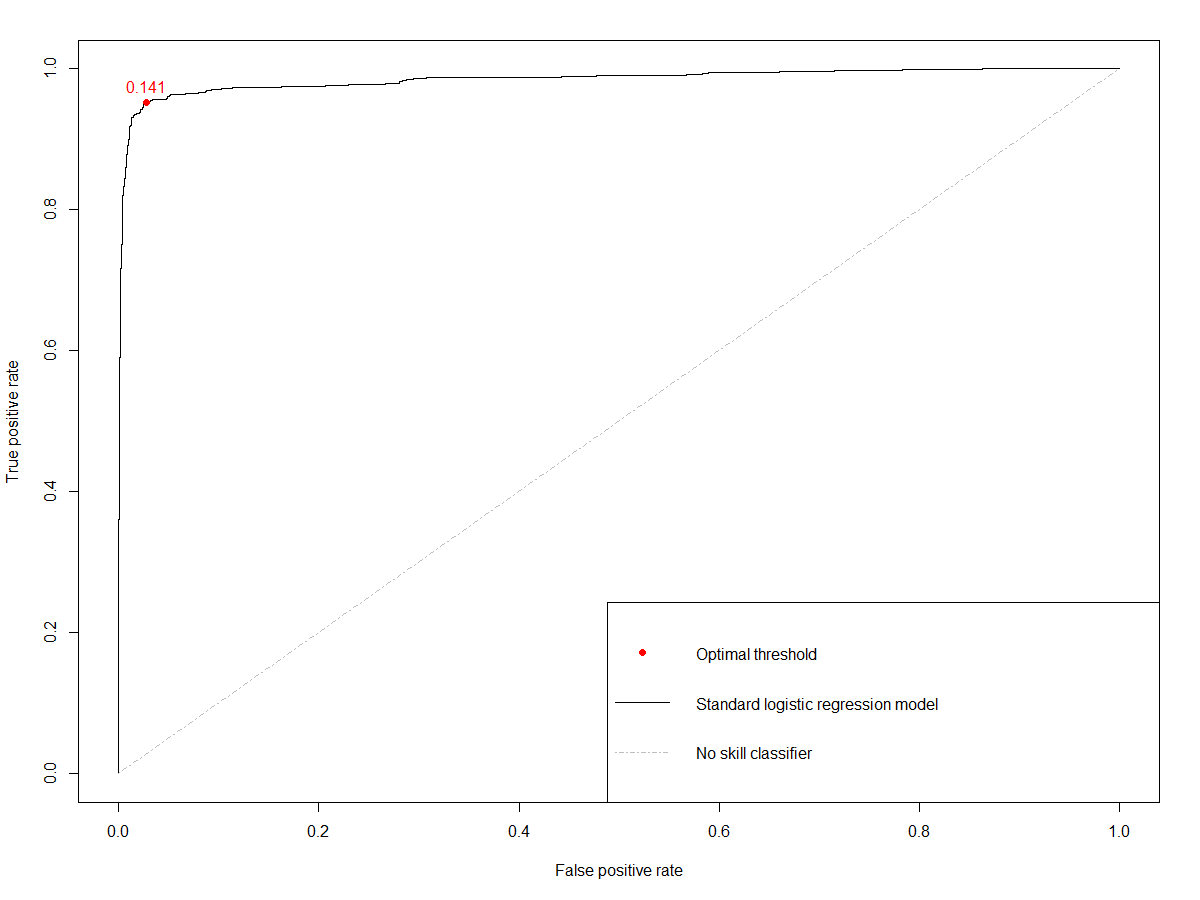
\includegraphics[scale=0.45]{fig/CH3/lasso_log_ROC_threshold_network.png}
		\caption{The ROC curve of the logistic regression model with an L1 penalty applied to the training network feature data set. Also, the plot provides the optimal threshold point (the threshold value that maximised the Geometric mean).}
		\label{fig:ch3_lr_thresh_roc_lasso_network}
	\end{center}	
\end{figure}

% Threshold moving - PR LR lasso network data
\begin{figure}
	\begin{center}
		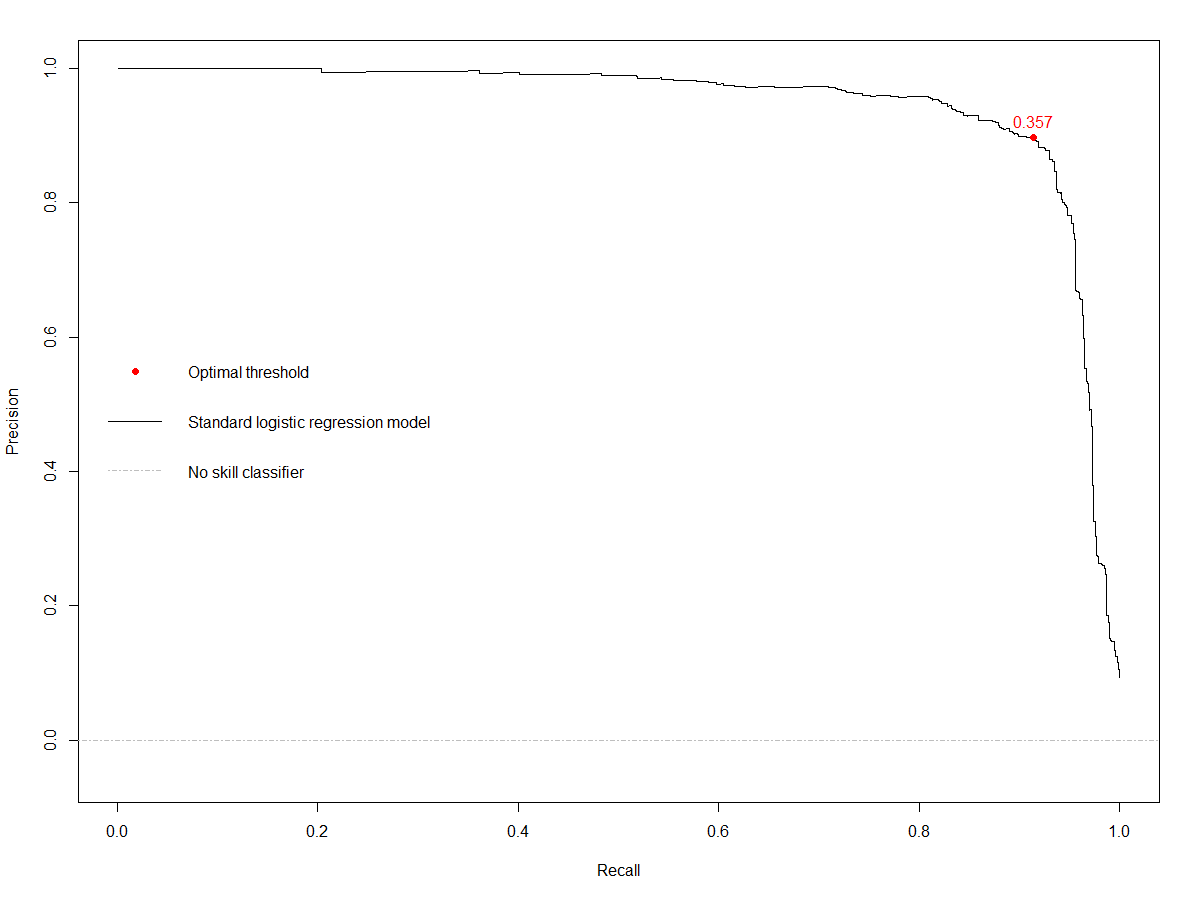
\includegraphics[scale=0.45]{fig/CH3/lasso_log_PR_threshold_network.png}
		\caption{The precision-recall curve of the logistic regression model with an L1 penalty applied to the training network feature data set. Also, the plot provides the optimal threshold point (the threshold value that maximised the F-measure).}
		\label{fig:ch3_lr_thresh_pr_lasso_network}
	\end{center}	
\end{figure}

% Neural networks
The second classifier is a \textit{ neural network}. The neural network model is a class of non-linear models used in supervised learning tasks \citep{et2020analytics}. Literature commonly compares the neural network model to that of the human brain. Although some terminology may overlap, one should not confuse its functioning with a biological neural network. As \citet{et2020analytics} said, the neural network is simply a mathematical model based on the idea that by the repeated iteration of translations of the input (with the depth of the network providing the number of repetitions) and specification of the calculation performed in each cell (node), we create a non-linear function of the input/predictor space which maps to the output. A more formal definition of a neural network, specifically a standard \textit{feed-forward neural network}, is as follows (adopted from \citep{et2020analytics}:

Let $a^l_j$ denote the $j^{th}$ node on $l^{th}$ layer of a standard feed-forward neural network, then the network structure can be written as an updating equation (in vector form):

$$\boldsymbol{a}^l = \sigma_l(\boldsymbol{W^T_l}\boldsymbol{a}^{l-1}+\boldsymbol{b}^l);\; l = 1,2,\ldots$$

where  $\boldsymbol{a}^l = [a^l_1,a^l_1,\ldots,a^l_j]^T$ denote vectors of activations. The parameters of the model are summarised in the weight matrices $\boldsymbol{W_l} = (w^l_{kj})$, where $w^l_{kj}$ is the $kj$-th weight paramter linking the $k$-th node in layer $l-1$ and $j$-th node in layer $l$. The bias vectors are denoted by $\boldsymbol{b}^l = [b^l_1,b^l_2,\ldots,b^l_j]^T$, and the initial values(s) for the equation is $\boldsymbol{a}^0 = \boldsymbol{x}_i$. Lastly, the $\sigma(.)_l$ denotes the activation function on layer $l$.

The above equation has the potential to emulate highly non-linear functions in the predictors. Also, increasing the number of nodes or layers within the equation increases the number of model parameters, and as a result, increases the models' complexity. As with the logistic regression model, in which the Equation \ref{ch3_log_lik_eq} needed to be maximised to obtain suitable weights for the model, so too does a neural network model need some optimisation technique to estimate appropriate weights within $\boldsymbol{W_l}$. \textit{Gradient descent} (or variants thereof) combined with \textit{backpropagation} is used to fit neural networks. Gradient descent is a numerical technique for finding extrema (such as Newton's method). The fundamental idea behind gradient descent is for each iteration, the algorithm tries to ``step'', with a certain \textit{magnitude}, in the \textit{direction} that improves the cost function. Both the direction and magnitude of the step-size are based on the cost function gradient given a set of inputs. On the other hand, backpropagation is an algorithm for calculating the gradient of a cost function with respect to variables of a model. Therefore, during the neural networks' training, the gradient for each weight in the network is calculated using backpropagation. After that, gradient descent uses the gradient to update the models' weights. The project will not provide the mathematical formulations of gradient descent and backpropagation; however, \citet*{nielsen2015neural} gives a thorough explanation of each.

Unlike the logistic regression model, the neural network model can not take categorical features as inputs. The neural networks can only take numerical predictors. As mentioned before, luckily, this is not a problem since all three structured data sets had numerical predictors. Standardising the predictor variables was the only data pre-processing necessary. This data pre-processing step was done due to the predictors' different units of measures. It is highly recommended that before implementing any neural network, one should ensure the same scales across all input variables \citep*{bishop1995neural}. The project defined two different neural networks in the project. Both models were standard feed-forward neural networks with a \textit{single} hidden layer. Based on the networks architecture, the only difference was the \textit{number of nodes} defined in the hidden layer. The first model had 8 hidden neurons and the second model had 64 hidden neurons. Architecturally, the number of hidden nodes in the hidden layer was the only difference. The activation function applied in the hidden layer and output layer of the models were the \textit{rectified linear unit} (ReLU) and \textit{soft-max} activation functions. The ReLU activation  function is a very popular activation function to use within hidden layers. ReLU's piecewise linear function provides a lot of desirable properties of a linear function when training a neural network using backpropagation \citep*{goodfellow2017deep}. However, the choice of the hidden layer activation function for neural networks becomes more significant when the depth of the network increases tremendously (as with \textit{deep learning} models) \citep{et2020analytics}. Therefore, the ReLU activation function will be sufficient for the hidden layers of the project neural network models. In terms of the activation function used in the output layer, we need to choose an activation function that matches the range of the encoded outputs due to the problem being a classification task \citep{et2020analytics}. It is useful to ensure that the output layer behaves like a \textit{distribution}, and therefore, the soft-max activation function was chosen. The cost function defined in training the neural networks was the so-called \textit{cross-entropy error}. This cost function is desirable since the gradient of the cross-entropy function w.r.t the model's parameters are less likely to ``bottoming out'' when it's far from a global solution \citep{et2020analytics}. The chosen optimiser used for each model was the \textit{adam} optimiser. The adam optimiser is an extension of the stochastic gradient descent learning algorithm, which takes as input three hyper-parameters: \textit{batch size}, \textit{epochs}, and  \textit{learning rate} $\nu$. There is no defined process in choosing the batch size or training epochs \citep{bengio2012practical, masters2018revisiting}. Choosing large batch sizes provides the learning algorithm with more training examples, which provides a more accurate estimate of the cost functions error gradient. Therefore, it is more likely that the weights of the network will be adjusted correctly so that the performance of the model increases. The drawback of choosing a large batch size (like in batch size gradient decent) is that the cost functions error gradient becomes highly dependent on the training samples used (which can negatively impact the model's generalisation). Alternatively, using small batch sizes results in less accurate estimates of the error gradient, which provides a ``noisy'' update to the weights. These noisy updates can result in faster learning and sometimes more robust models \citep*{jason2019batch}. On the other hand, the training epochs is the number of full pass overs of the training dataset. A small number of epochs is computationally beneficial, however, you run the risk of the algorithm not completely reaching an extremum. Depending on the problem, choosing a very high number of training epochs is also not ideal since it can lead to overfitting the model. This begin said the batch size and epoch values chosen for both models were 100 and 20, respectively. Also, 0.001 was chosen as the \textit{learning rate} for the adam optimiser (the optimisers default value).

As mentioned before, regularisation is a useful technique in controlling a models complexity. Some of the most straightforward neural network architectures are able to construct complex non-linear functions. Therefore, it is essential to apply some form of regularisation mechanism, in which we can ensure that our model has generalised to some degree. \textit{L2 regularisation} was the chosen regularisation method for the neural network models. As mentioned with the logistic regression model, the implication of adopting L2 regularisation is that an additional hyper-parameter, $\lambda$, needs to be specified. The project determined an appropriate value for $\lambda$ each neural network model by using a validation set (hold-out set). Therefore, 70\% was used for training (fitting) the models for each structured training data set, and 30\% was used for validation. Figure \ref{fig:ch3_nn_validation_mod1_network} and Figure \ref{fig:ch3_nn_validation_mod2_network}  illustrate the process of finding the best approximate $\lambda$ value for the (8)-network and (64)-network, respectively, using the network feature data set. Two plots are shown in the Figure. The left plot shows the validation and training errors for $\lambda \in [0,1]$. The right plot also shows the validation and training errors but for a more focused set of $\lambda$ values. Also, the value of $\lambda$, which produced a minimum validation error, is shown by the red dashed line. This type plot was constructed for each of the two neural network models (the (64)-network and the (8)-network) for each structured training data set (network feature, transactional feature, and combined.). In appendix \ref{app_2} Figures \ref{fig:ch3_nn_validation_mod1_trans} and \ref{fig:ch3_nn_validation_mod2_trans} show the best approximated $\lambda$ values for the transactional feature data set for the (8)-network and (64)-network models, respectively. Also, Figures \ref{fig:ch3_nn_validation_mod1_all} and \ref{fig:ch3_nn_validation_mod2_all} show the best approximated $\lambda$ values for the combined feature data set for the (8)-network and (64)-network models, respectively.

% [conclusion - modelling]
This section explained the modelling procedure implemented in the project. For both the logistic regression and neural network models: the data pre-processing was done, the models' architectures were defined, and hyper-parameter tuning was performed to find appropriate values for the models hyper-parameters. The final step in the modelling procedure was choosing which models would most likely deliver good out-of-sample performance based on the training results. The out-of-sample performance of the model will be estimated using test data sets (``unseen'' data sets). Three models were chosen to be evaluated against the test data sets (test network feature data set, test transactional feature data set, and test combined feature data set). The first model was the logistic regression model with L1 regularisation. The threshold value chosen for the model was based on the optimal threshold according to its ROC curve. The second model was identical to the first. However, the threshold value was chosen according to the optimal threshold value calculated from its precision-recall curve. The final model was the (8)-network model. The (8)-network model was preferred over the (64)-model because both yielded similar validation errors for each structured data set. Figure \ref{fig:ch3_nn_validation_compare_network} illustrates this point for the network feature data set. Figure \ref{fig:ch3_nn_validation_compare_trans} and Figure \ref{fig:ch3_nn_validation_compare_combined} in appendix \ref{app_1} show a similar result. Therefore, as \citet{james2013introduction} recommends, it is better to choose the simpler model that delivers a similar performance to the complex model. From here onwards, the project will refer to the first model as ``LR-ROC'', the second model as ``LR-PR'' and the third model as ``(8)-NN''. Also, Table \ref{tab:ch3_model_summary} provides a summary of the three models and how they were configured for each data set. The results, after testing the models on the test data sets, are presented in section \ref{ch3_sub_heading_results}.

% validation curves NN -  (8)-network data
\begin{figure}
	\begin{center}
		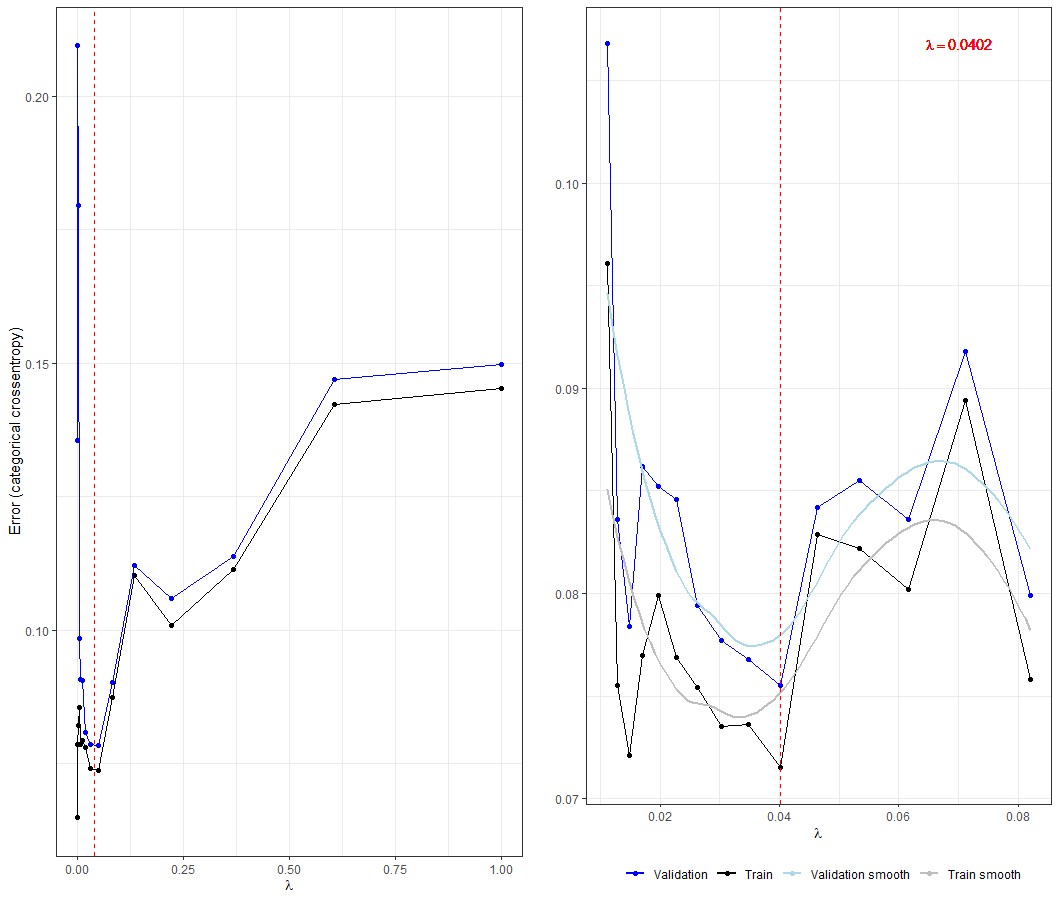
\includegraphics[scale = 0.55]{fig/CH3/network_mod_1_lambda_plot.png}
		\caption{The plot illustrates the process of selecting the best approximate $\lambda$ value for the (8)-network model applied to the network feature data set. (left) The training and validation set errors for a range of $\lambda$ values. (right) The training and validation set errors for a more specific range of $\lambda$ values. The training and validation error smooth curves are auxiliary curves to help view the curve patterns. Also, the $\lambda$ value that produced the minimum validation error is shown in both plots.}
		\label{fig:ch3_nn_validation_mod1_network}
	\end{center}	
\end{figure}

% validation curves NN -  (64)-network data
\begin{figure}
	\begin{center}
		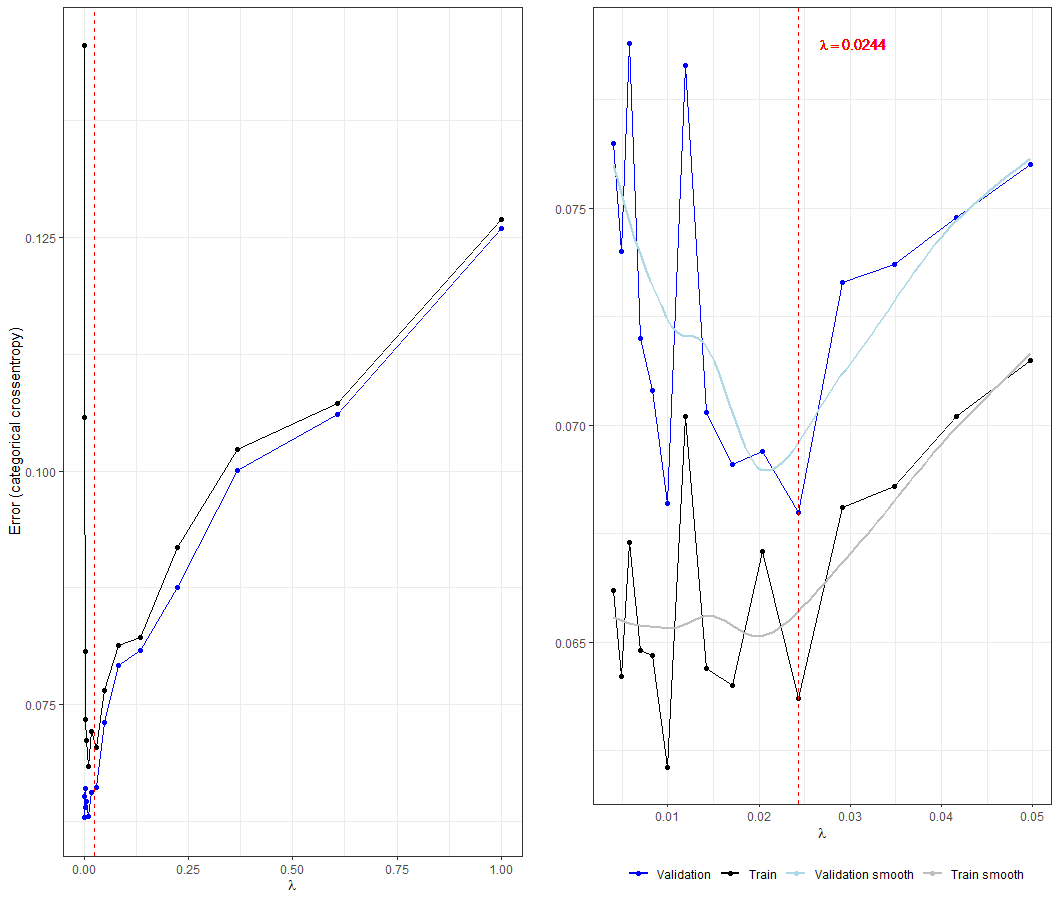
\includegraphics[scale = 0.5]{fig/CH3/network_mod_2_lambda_plot.png}
		\caption{The plot illustrates the process of selecting the best approximate $\lambda$ value for the (64)-network model applied to the network feature data set. (left) The training and validation set errors for a range of $\lambda$ values. (right) The training and validation set errors for a more specific range of $\lambda$ values. The training and validation error smooth curves are auxiliary curves to help view the curve patterns. Also, the $\lambda$ value that produced the minimum validation error is shown in both plots.}
		\label{fig:ch3_nn_validation_mod2_network}
	\end{center}	
\end{figure}

% validation curves comparison NN -  network data
\begin{figure}
	\begin{center}
		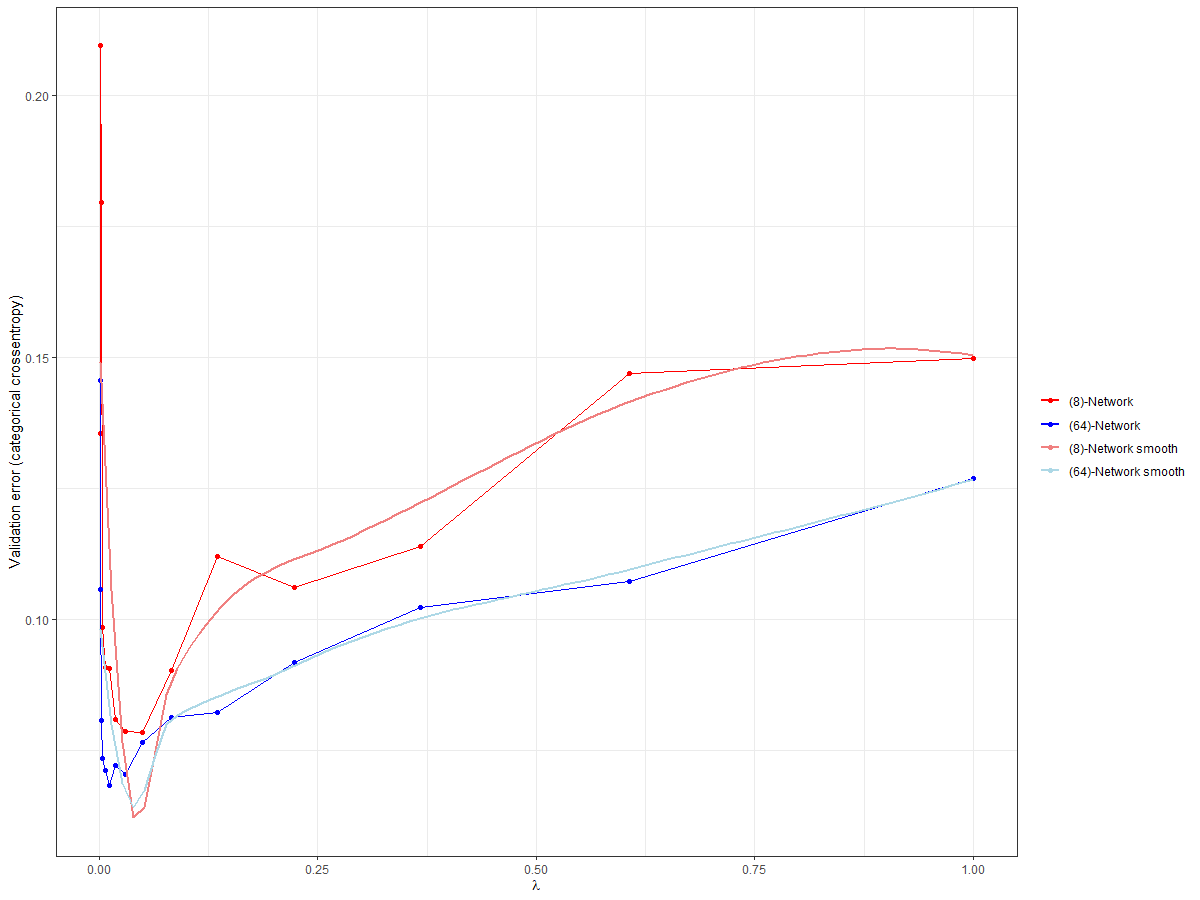
\includegraphics[scale = 0.5]{fig/CH3/model_comp_network_HL.png}
		\caption{The superimposed validation error curves of the (8)-Network and (64)-Network models and their smoothing curves for $\lambda \in [0,1]$. Both models were applied to the network features data set.}
		\label{fig:ch3_nn_validation_compare_network}
	\end{center}	
\end{figure}

% model summary table
\begin{table}
\resizebox{\columnwidth}{!}{%
\begin{tabular}{llclll}
\hline
\multicolumn{1}{c}{\textbf{\begin{tabular}[c]{@{}c@{}}Model \\ name\end{tabular}}} & \multicolumn{1}{c}{\textbf{\begin{tabular}[c]{@{}c@{}}Model \\ type\end{tabular}}} & \textbf{\begin{tabular}[c]{@{}c@{}}Regularisation \\ mechanism\end{tabular}} & \multicolumn{1}{c}{\textbf{\begin{tabular}[c]{@{}c@{}}Regularisation\\ factor\end{tabular}}}                                               & \multicolumn{1}{c}{\textbf{\begin{tabular}[c]{@{}c@{}}Additional \\ hyper-paramters\end{tabular}}}                                    & \multicolumn{1}{c}{\textbf{\begin{tabular}[c]{@{}c@{}}Additional \\ info\end{tabular}}}                                                                                                                                                                                                                                \\ \hline
LR-ROC                                                                             & \begin{tabular}[c]{@{}l@{}}Logistic \\ regression\end{tabular}                     & L1                                                                           & \begin{tabular}[c]{@{}l@{}}$\lambda_{network} = 0.003$;\\ $\lambda_{transactional} = 0.0003$;\\ $\lambda_{combined} = 0.0002$\end{tabular} & \begin{tabular}[c]{@{}l@{}}$\theta_{network} = 0.141$;\\ $\theta_{transactional} = 0.088$;\\ $\theta_{combined} = 0.159$\end{tabular} & \begin{tabular}[c]{@{}l@{}}The threshold was chosen according \\ to the optimal threshold on the ROC \\ curve.\end{tabular}                                                                                                                                                                                            \\ \hline
LR-PR                                                                              & \begin{tabular}[c]{@{}l@{}}Logistic \\ regression\end{tabular}                     & L1                                                                           & \begin{tabular}[c]{@{}l@{}}$\lambda_{network} = 0.003$;\\ $\lambda_{transactional} = 0.0003$;\\ $\lambda_{combined} = 0.0002$\end{tabular} & \begin{tabular}[c]{@{}l@{}}$\theta_{network} = 0.357$;\\ $\theta_{transactional} = 0.397$;\\ $\theta_{combined} = 0.462$\end{tabular} & \begin{tabular}[c]{@{}l@{}}The threshold was chosen according \\ to the optimal threshold on the \\ precision-recall curve.\end{tabular}                                                                                                                                                                               \\ \hline
(8)-NN                                                                        & \begin{tabular}[c]{@{}l@{}}Neural \\ Network\end{tabular}                          & L2                                                                           & \begin{tabular}[c]{@{}l@{}}$\lambda_{network} = 0.04$;\\ $\lambda_{transactional} = 0.002$;\\ $\lambda_{combined} = 0.03$;\end{tabular}    & \begin{tabular}[c]{@{}l@{}}Epochs = 20;\\ Batch size = 100;\\ $\nu$ = 0.001\end{tabular}                                              & \begin{tabular}[c]{@{}l@{}}Standard feed-forward neural network \\ with one hidden layer. The ReLU \\ activation function was applied in \\ the hidden layer and the soft-max\\ activation function was applied to \\ the output layer. Lastly, the  Adam \\ optimiser was used in training \\ the model.\end{tabular} \\ \hline
\end{tabular}
}
\caption{The Table provides a complete summary of the chosen models used to make predictions on each test data set. In addition, the hyper-parameters for each data set are also specified. Note that if the subscripts of the specific data set are not mentioned, then the specific hyper-parameter was kept the same for each data set.}
\label{tab:ch3_model_summary}
\end{table}

\section{Results}\label{ch3_sub_heading_results}

% Introduction to results section
The previous section explained the modelling procedure and how each model type was configured and constructed. Finally, the section concluded that three models (LR-ROC, LR-PR, and (8)-NN) were chosen to make predictions on unseen data. So far, the project has established an idea of each of the model's in-sample performance. However, this section aims to provide how the models performed out-of-sample.

% Introduction to the performances metrics used 
 The performance measures or metrics used to evaluate each data set's models were \textit{F1-score}, \textit{balanced accuracy}, and \textit{classification accuracy}. Although classification accuracy was included in the list of performance metrics, it is not an ideal classification performance metric if a data set is highly imbalanced \citep*{branco2015survey}. As mentioned before, approximately 1\% of all transactions are fraudulent, and approximately 5\% of all accounts have participated in money laundering activity. Therefore, the class distributions of the projects data sets are severely skewed. In such a case, the classification accuracy can be misleading due to the \textit{accuracy paradox} \citep{branco2015survey}. This phenomenon can be explained at the hand of the following toy example. Suppose we have a data set with a 1:100 class imbalance, ``0'' representing the majority class and ``1'' representing the minority class. If a naive model predicts ``0'' for all observations in the test set, then the model would have attained a classification accuracy of 99\%. On the surface, this seems like a very impressive result. However, one can easily forget that the naive classifier predicted only the majority class. This raises the question of whether the model's performance is as impressive as the classification accuracy depicts. In the example, the classification accuracy is correct. However, it is the analyst intuition, thinking the model actually ``learnt'', which is the real pitfall. 
 
% f1 - performance metric
Therefore, it is essential to define other performance metrics that can better cope with imbalanced data set such as the F1-score and balanced accuracy. The F1-score ($F_1$) is calculated as follows:

\begin{equation}
    F_1 = \frac{2 \times TP}{2 \times TP + FP + FN}
\label{ch3_f1_eq}
\end{equation} 

Where $FP$ is the false-positives - honest accounts predicted as fraudulent accounts, $TP$ is the true-positives - correctly predicted money laundering accounts, and $FN$ is the false-negatives - a money laundering account predicted as an honest account. The F1-score is also defined of as the harmonic mean of $precision = \frac{TP}{TP+FP}$ and $recall = \frac{TP}{TP + FN}$ \citep{james2013introduction}. Precision and recall are not much affected by heavily skewed data (as seen by their expressions). Therefore, the F1-score should be an appropriate performance metric since it combines precision and recall values into a single metric. On the other hand, balanced accuracy is calculated as follows:

$$Balanced\;accuracy = \frac{\frac{TP}{T_{P}} = \frac{TN}{T_{N}}}{2} $$

% balanced acc - performance metric
Where $T_{P}$ is the total positives and $T_{N}$ is the total negatives. By taking the average of the total number of positive cases correctly predicted ($sensitivity = recall$) and the total number of negative cases correctly predicted ($specificity = \frac{TN}{T_{N}}$), we are left with a measure illustrating the prediction performance of \textit{both} classes. For example, if we consider a naive binary classifier that only predicts the majority class (``0''), we will obtain a high value for specificity, however, it will obtain a very low value for sensitivity (representing the prediction accuracy of the minority class ``1'') resulting in a lower overall average between the two metrics. 
% results interpreation
Table \ref{tab:ch3_model_results} provides a summary of each models performance on each test data set. Classification accuracy was included; however one should be cautious when jumping to conclusions using this metric due to the aforementioned reasons. It is also important that note that a naive classifier, which only predicts the majority class (\texttt{is\_fraud} = False), would have obtained a classification accuracy of \textbf{94.5\%} on each test set. Models that received their inputs from the network feature data set will be referred to as the ``network feature models''. The same applies to the transactions and combined feature data sets. Starting with the F1-score metric, on average, the network feature models scored \textbf{0.371} higher than the transactional feature models. The combined feature models average F1-score performance was slightly better (0.01) than the average F1-score of the network feature models. Generally, the (8)-NN model delivered the highest F1-scores, however, on average, the LR-PR model was the better model. Looking at the balanced accuracy measurement, very high values were recorded for the network feature models. It was unexpected that each network feature model outperformed each respective combined feature model i.t.o balanced accuracy. On average, the transactional feature models scored much lower (\textbf{0.21}) than the network feature models. Overall, the two logistic regression models, LR-ROC and LR-PR, outperformed the (8)-NN model on balanced accuracy scores. Specifically, on average, the LR-ROC model outperformed the other models on the balanced accuracy metric. The defined model metrics help analyse the performance of each model, given the different set of input features. However, looking at each models \textit{confusion matrix} can also provide insight into the models' performance. The confusion matrices for all models for each data set is provided in appendix \ref{app_1}. Some noticeable findings were that all the network feature models (Tables \ref{tab:ch3_cm_LR_ROC_network}, \ref{tab:ch3_cm_LR_PR_network}, and \ref{tab:ch3_cm_nn_network}) had a relatively low number of false negatives. On the other hand, the transactional feature models had higher false positives (Table \ref{tab:ch3_cm_LR_PR_trans} and Table \ref{tab:ch3_cm_LR_PR_network}) and higher false negatives (Table \ref{tab:ch3_cm_LR_ROC_trans}). The confusion matrices of the combined feature models were very similar to the network feature models. From a practical point of view, it would be valuable for a commercial bank to pay close attention to the false positive accounts since these accounts seem to exhibit similar behaviour to the money laundering accounts and, therefore, are a higher risk.  

Finally, Figure \ref{fig:ch3_final_results_bar}, Figure \ref{fig:ch3_final_results_f1_density}, and Figure \ref{fig:ch3_final_results_balanced_acc_density} were included as visual illustrations of the results displayed in Table \ref{tab:ch3_model_results}. Looking at Figure \ref{fig:ch3_final_results_f1_density} and Figure \ref{fig:ch3_final_results_balanced_acc_density} it is very noticeable that the the network feature models performed much better i.t.o F1-score and balanced accuracy than the transnational feature models. The combined feature models scored slightly better than the network feature models in F1-score. Even though the network feature models obtained higher balanced accuracy scores than the combined feature models, the balanced accuracy distribution of the combined feature models was much narrower than that of the network feature models.  

% Model/Data set final results
\begin{table}
\begin{tabular}{cllll|l}
\hline
\textbf{\begin{tabular}[c]{@{}c@{}}Performance \\ metric\end{tabular}}        & \multicolumn{1}{c}{\textbf{\begin{tabular}[c]{@{}c@{}}Data \\ set\end{tabular}}} & \multicolumn{1}{c}{\textbf{LR-ROC}} & \multicolumn{1}{c}{\textbf{LR-PR}} & \multicolumn{1}{c|}{\textbf{(8)-NN}} & \multicolumn{1}{c}{\textbf{Average}} \\ \hline
\multirow{3}{*}{Accuracy}                                                     & Network feature                                                                  & 0.955                               & 0.978                              & $0.986^*$                            & 0.973                                \\
                                                                              & Transactional feature                                                            & 0.846                               & $0.95^*$                           & 0.935                                & 0.91                                 \\
                                                                              & Combined                                                                         & 0.953                               & 0.95                               & $0.988^*$                            & 0.964                                \\ \hline
\multicolumn{1}{l}{}                                                          & \textbf{Average:}                                                                & 0.918                               & 0.959                              & 0.97                                 &                                      \\ \hline
\multirow{3}{*}{F1-score}                                                     & Network feature                                                                  & 0.701                               & 0.826                              & $0.885^*$                            & 0.804                                \\
                                                                              & Transactional feature                                                            & 0.361                               & $0.577^*$                          & 0.361                                & 0.433                                \\
                                                                              & Combined                                                                         & 0.693                               & 0.857                              & $0.892^*$                            & 0.814                                \\ \hline
\multicolumn{1}{l}{}                                                          & \textbf{Average:}                                                                & 0.585                               & 0.753                              & 0.713                                &                                      \\ \hline
\multirow{3}{*}{\begin{tabular}[c]{@{}c@{}}Balanced \\ accuracy\end{tabular}} & Network feature                                                                  & 0.957                               & 0.969                              & $0.973^*$                            & 0.966                                \\
                                                                              & Transactional feature                                                            & $0.82^*$                            & 0.797                              & 0.652                                & 0.756                                \\
                                                                              & Combined                                                                         & $0.956^*$                           & 0.952                              & 0.954                                & 0.954                                \\ \hline
\multicolumn{1}{l}{}                                                          & \textbf{Average:}                                                                & 0.911                               & 0.906                              & 0.86                                 &                                      \\ \hline
\end{tabular}
\caption{A summary of the models (LR-ROC, LR-PR, and (8)-NN) results when applied to each test data set (network feature, transactional, and combined). The performance evaluation metrics were classification accuracy, F1-score, and Balanced accuracy metrics. The model that performed the best for a specific data set was indicated using the asterisk symbol ($*$). The average performance is shown on each data set's far most right column. In addition, the average performance for each model is shown in the rows between the metrics.}
\label{tab:ch3_model_results}
\end{table}

% Summary result figures - bar
\begin{figure}
	\begin{center}
		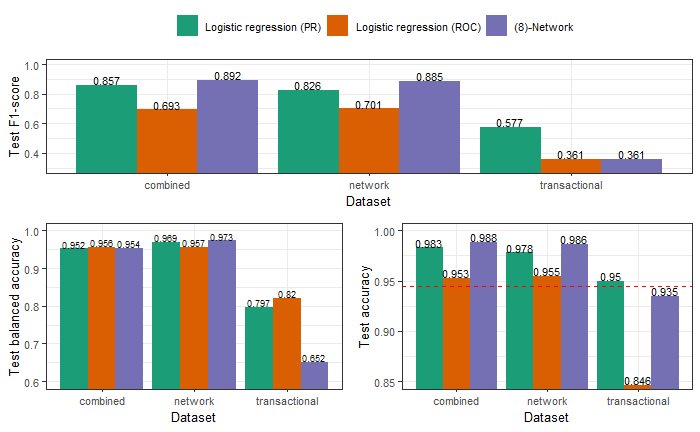
\includegraphics[scale = 0.8]{fig/CH3/data_sets_summary_bar.png}
		\caption{The plot shows a visual representation summarising the performance of each of the models on each test data set. (top) The F1-score for each model applied to each test data set. (bottom-left) The balanced accuracy score for each model applied to each test data set. (bottom-right) The classification accuracy for each model applied to each test data set. Also, the red dashed line indicates the classification accuracy of a naive classifier, which only predicted the majority class.}
		\label{fig:ch3_final_results_bar}
	\end{center}	
\end{figure}

% Summary result figures - density f1
\begin{figure}
	\begin{center}
		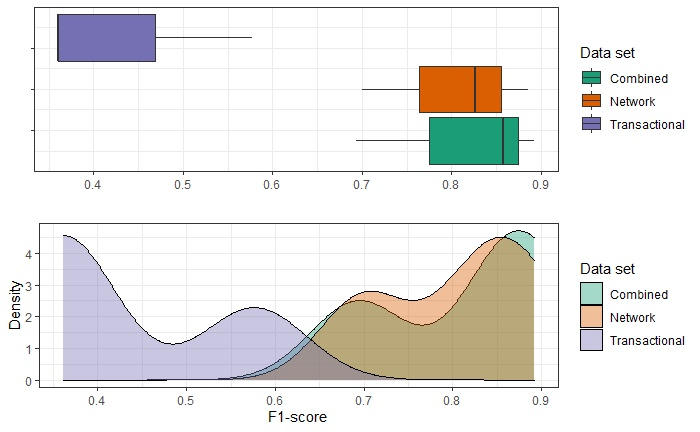
\includegraphics[scale = 0.6]{fig/CH3/data_sets_test_f1_density_LI.jpg}
		\caption{A visual representation of the tested models F1-score distribution grouped by the given input data set.}
		\label{fig:ch3_final_results_f1_density}
	\end{center}	
\end{figure}

% Summary result figures - density balanced acc
\begin{figure}
	\begin{center}
		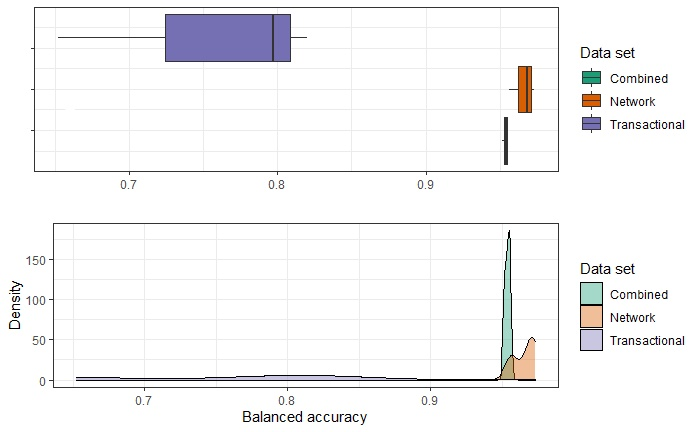
\includegraphics[scale = 0.6]{fig/CH3/data_sets_balance_acc_density_LI.jpg}
		\caption{A visual representation of the tested models balanced accuracy distribution grouped by the given input data set.}
		\label{fig:ch3_final_results_balanced_acc_density}
	\end{center}	
\end{figure}



% Ask Et: Should I include examples of the each input file (if needed)?
% Should I go into the details of how the simulator was run (instructions) virtual linux environment python files, bash files, etc?
